\documentclass[12pt]{article}
\usepackage{fullpage,url,amssymb,epsfig,color,xspace,tikz,amsmath, amsthm}
\usetikzlibrary{matrix,backgrounds}

\begin{document}
    
\begin{center}
    \textbf{\huge Midterm Review}
\end{center}

\section{Input/Output}
\begin{enumerate}
    \item Write a function that reads in a sequence of strings from a file. The file name is passed through 
    command line. The function should print every second string to standard out(on a line by itself).
    \item What will the code below print?
        \begin{verbatim}
#include <iostream>
using namespace std;
    
int main() {
  int num;
  while(cin) {
    cin >> num;
    cout << num << endl;
  }
}
    
Input:
1EOF
        \end{verbatim}
\end{enumerate}

\section{Shell}
\begin{enumerate}
    \item \begin{verbatim}
echo *
echo '*'
echo "*"
echo '${HOME}'
echo "${HOME}"
echo '"${HOME}"'
echo "'${HOME}'"
    \end{verbatim}
    \item Store all the names of .cc files to assignlist.txt
    \item Count the number of words in all .cc files(wc is the command for counting the number of words)
\end{enumerate}

\section{Pointers \& References}
\begin{enumerate}
    \item \begin{verbatim}
#include <iostream>
using namespace std;

int main() {
  int a = 0;
  int b = 1;
  int *p1 = &a;
  int *p2 = &b;
  p1 = *&*&*&p2;
  cout << *p1 << endl;
  *p1 = 2;
  cout << *p2 << endl;
  p1 = &a;
  int **p3 = &p1;
  *p3 = p2;
  cout << **p3 << endl;
}
    \end{verbatim}
    \item What are the differences and similarities between references and pointers?
\end{enumerate}

\section{Linked List}
\begin{enumerate}
    \item You are given two equal sized non-empty linked lists representing two non-negative integers. 
    The digits are stored in reverse order and each of their nodes contain a single digit. 
    Add the two numbers and return it as a linked list. You may assume the two numbers do 
    not contain any leading zero, except the number 0 itself.
    \begin{verbatim}
Input: (2 -> 4 -> 3) + (5 -> 6 -> 4)
Output: 7 -> 0 -> 8
Explanation: 342 + 465 = 807
    \end{verbatim}
    Node *add(Node *n1, Node *n2) {}
\end{enumerate}

\section{Stack}
\begin{enumerate}
    \item Make sure know how to implement stack using linked list and vector array
    \item Use stack to reverse a word.
    \item Can you name one application of stack?
    \item Suppose you are asked to implement a back/forward button for a browser. How would you do it?
\end{enumerate}

\section{Queue}
\begin{enumerate}
    \item Implement queue using the struct below where 
    \begin{itemize}
        \item arr has fixed length "size"
        \item frt stores the index of first element
        \item last stores the index of last element
        \item the next element of arr[size - 1] is arr[0]
    \end{itemize}
    \begin{verbatim}
struct Queue {
  int size;
  int frt;
  int last;
  int *arr;
};
void init(Queue &q, int size);
//if queue is full, replace the oldest element in the queue
void add(Queue &q, int val);
void remove(Queue &q);
void print(Queue &q);
    \end{verbatim}    
    For example,\\
    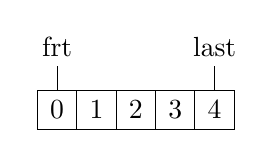
\begin{tikzpicture}[
        array/.style={matrix of nodes,nodes={draw, minimum size=7mm},column sep=-\pgflinewidth, row sep=0.5mm, nodes in empty cells,
        row 1/.style={nodes={minimum size=5mm}}}]
        \matrix[array] (array) {
        0 & 1 & 2 & 3 & 4 \\};
        \draw (array-1-1.north)--++(90:3mm) node [above] (first) {frt};
        \draw (array-1-5.north)--++(90:3mm) node [above] (first) {last};
    \end{tikzpicture}\\
    add(q, 5)\\
    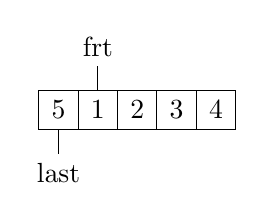
\begin{tikzpicture}[
        array/.style={matrix of nodes,nodes={draw, minimum size=7mm},column sep=-\pgflinewidth, row sep=0.5mm, nodes in empty cells,
        row 1/.style={nodes={minimum size=5mm}}}]
        \matrix[array] (array) {
        5 & 1 & 2 & 3 & 4 \\};
        \draw (array-1-2.north)--++(90:3mm) node [above] (first) {frt};
        \draw (array-1-1.south)--++(-90:3mm) node [below] (first) {last};
    \end{tikzpicture}
    \item Advantages of implementing priority queue using heap
\end{enumerate}

\section{Testing}
\begin{enumerate}
    \item what is the definition of white-box testing
    \item what is the definition of black-box testing
\end{enumerate}


\section{Trees}
\begin{enumerate}
    \item Implement a function which calcualtes a binary tree's height.
    \item An array representation of a binary tree is defined as:
    \begin{itemize}
        \item root is at index 0,
        \item if a node has index $i$ and both children exsit, the left child is at index $2 * i + 1$, 
        the right child at index $2 * i + 2$
        \item if a child of a node does not exist, it has the value 0 if the index is valid
    \end{itemize}
    Implement has which returns true if the value that we look up exsits otherwise false. 
    \item Make sure you know how heap works. 
\end{enumerate}
\end{document}